\chapter{Analysis and results}
\label{ch:results}

\section{Exploratory Promenade results}
The three original daily/comparator logs provide the descriptive results in Table~\ref{tab:promenade}. These are individual stochastic runs, separate from the five-replication means reported later.
\begin{table}[htbp]\centering\small
\begin{tabular}{lrrr}\hline
Metric (minutes) & Nov. 1 literature & Nov. 8 literature & Nov. 1 original\\\hline
Cases & 271 & 238 & 271\\
Mean block duration & 62.33 & 59.59 & 84.95\\
Median & 55.62 & 57.34 & 64.37\\
90th percentile & 72.48 & 72.83 & 80.12\\
Maximum & 434.83 & 116.70 & 421.95\\\hline
\end{tabular}
\caption{Paired simulated in-block/off-block durations checked in Promenade. Original denotes original service functions inside the same demand adapter.}\label{tab:promenade}
\end{table}

Every paired analysis has zero unmatched starts. Differences establish sensitivity to timing assumptions, not empirical improvement. In particular, inherited policy affects the long tail. Figure~\ref{fig:promenade} preserves an actual Promenade timing view.
\begin{figure}[htbp]\centering
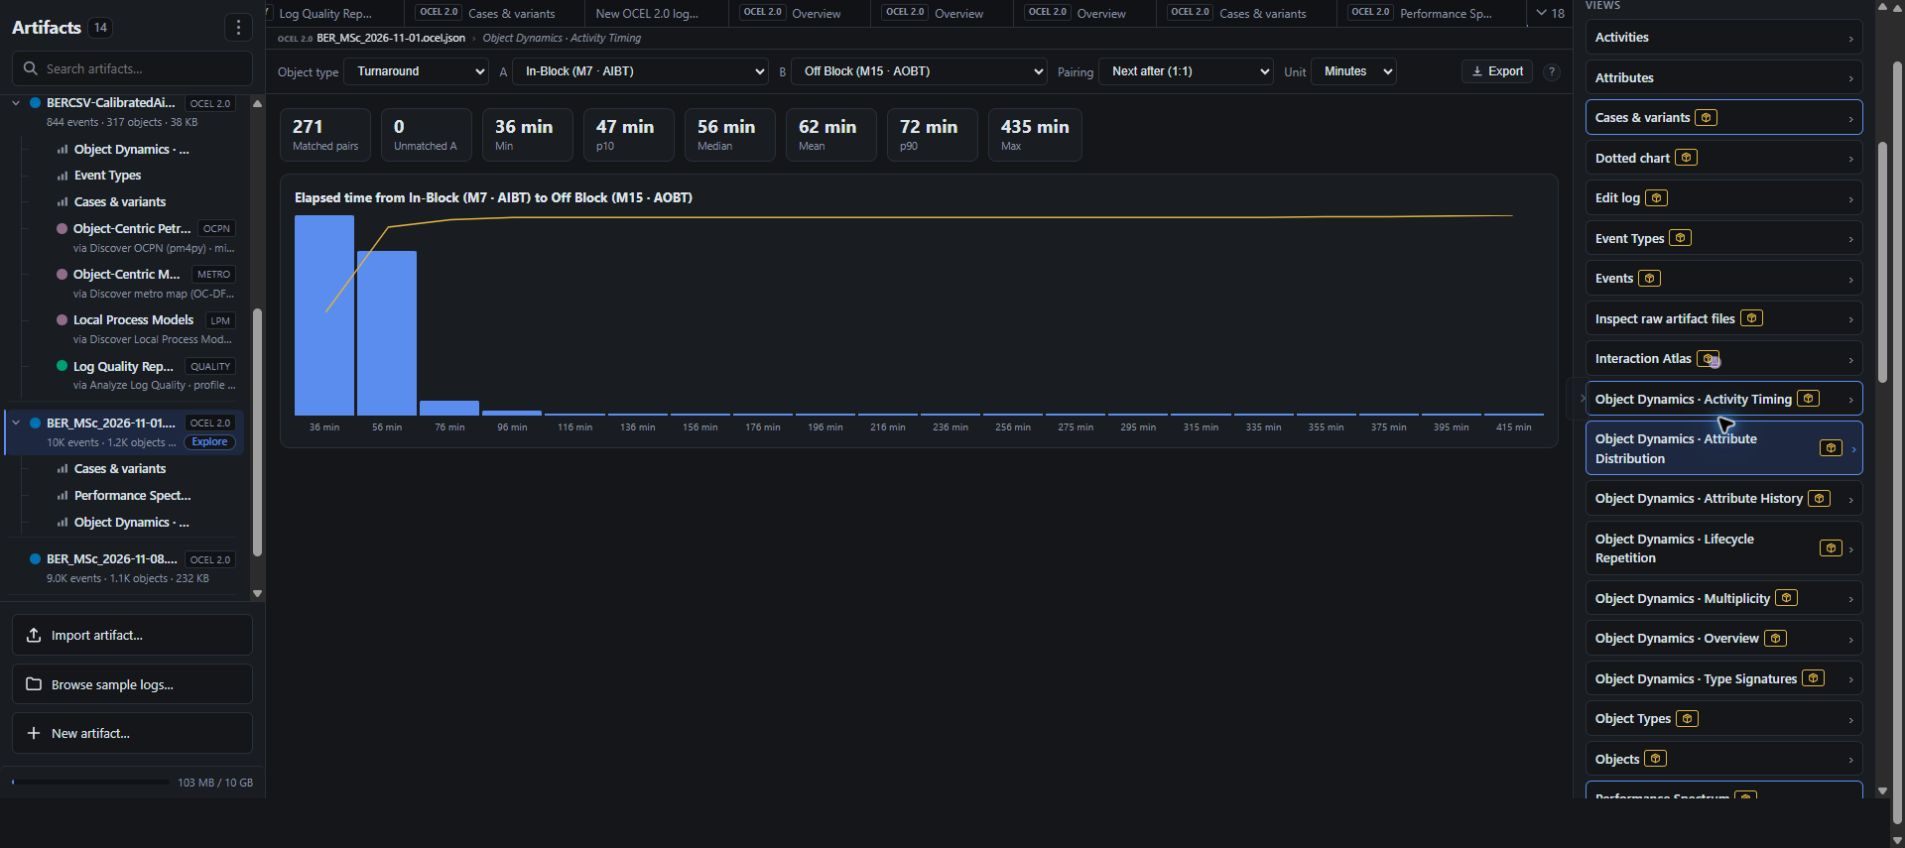
\includegraphics[width=\textwidth]{study_promenade_timing.jpg}
\caption{Promenade Object Dynamics/Activity Timing view of the 1 November literature-timing log. The data are generated simulation events.}\label{fig:promenade}
\end{figure}

\section{Resource queues and handling dependencies}
In the individual literature-timing runs, mean fuel-dispatch waiting is 3.785 minutes on 1 November and 1.255 minutes on 8 November. Cleaning-team waiting is 0.018 and approximately zero minutes; tug-allocation waiting is 0.033 and approximately zero. The 1 November 90th-percentile fuel waiting time is 14.20 minutes, with a maximum of 38.28 minutes.

Nevertheless, the cabin/boarding branch is last ready in 230 of 271 turnarounds (84.9\%) and 192 of 238 (80.7\%). Fuel is last in only 21 and 10 cases; baggage handling is last in 20 and 36. Thus the largest local queue is not automatically the branch governing final readiness. Fuel waiting can overlap continuing cabin work. These counts describe synchronization outcomes, not a proof of causal dominance.
\begin{figure}[htbp]\centering
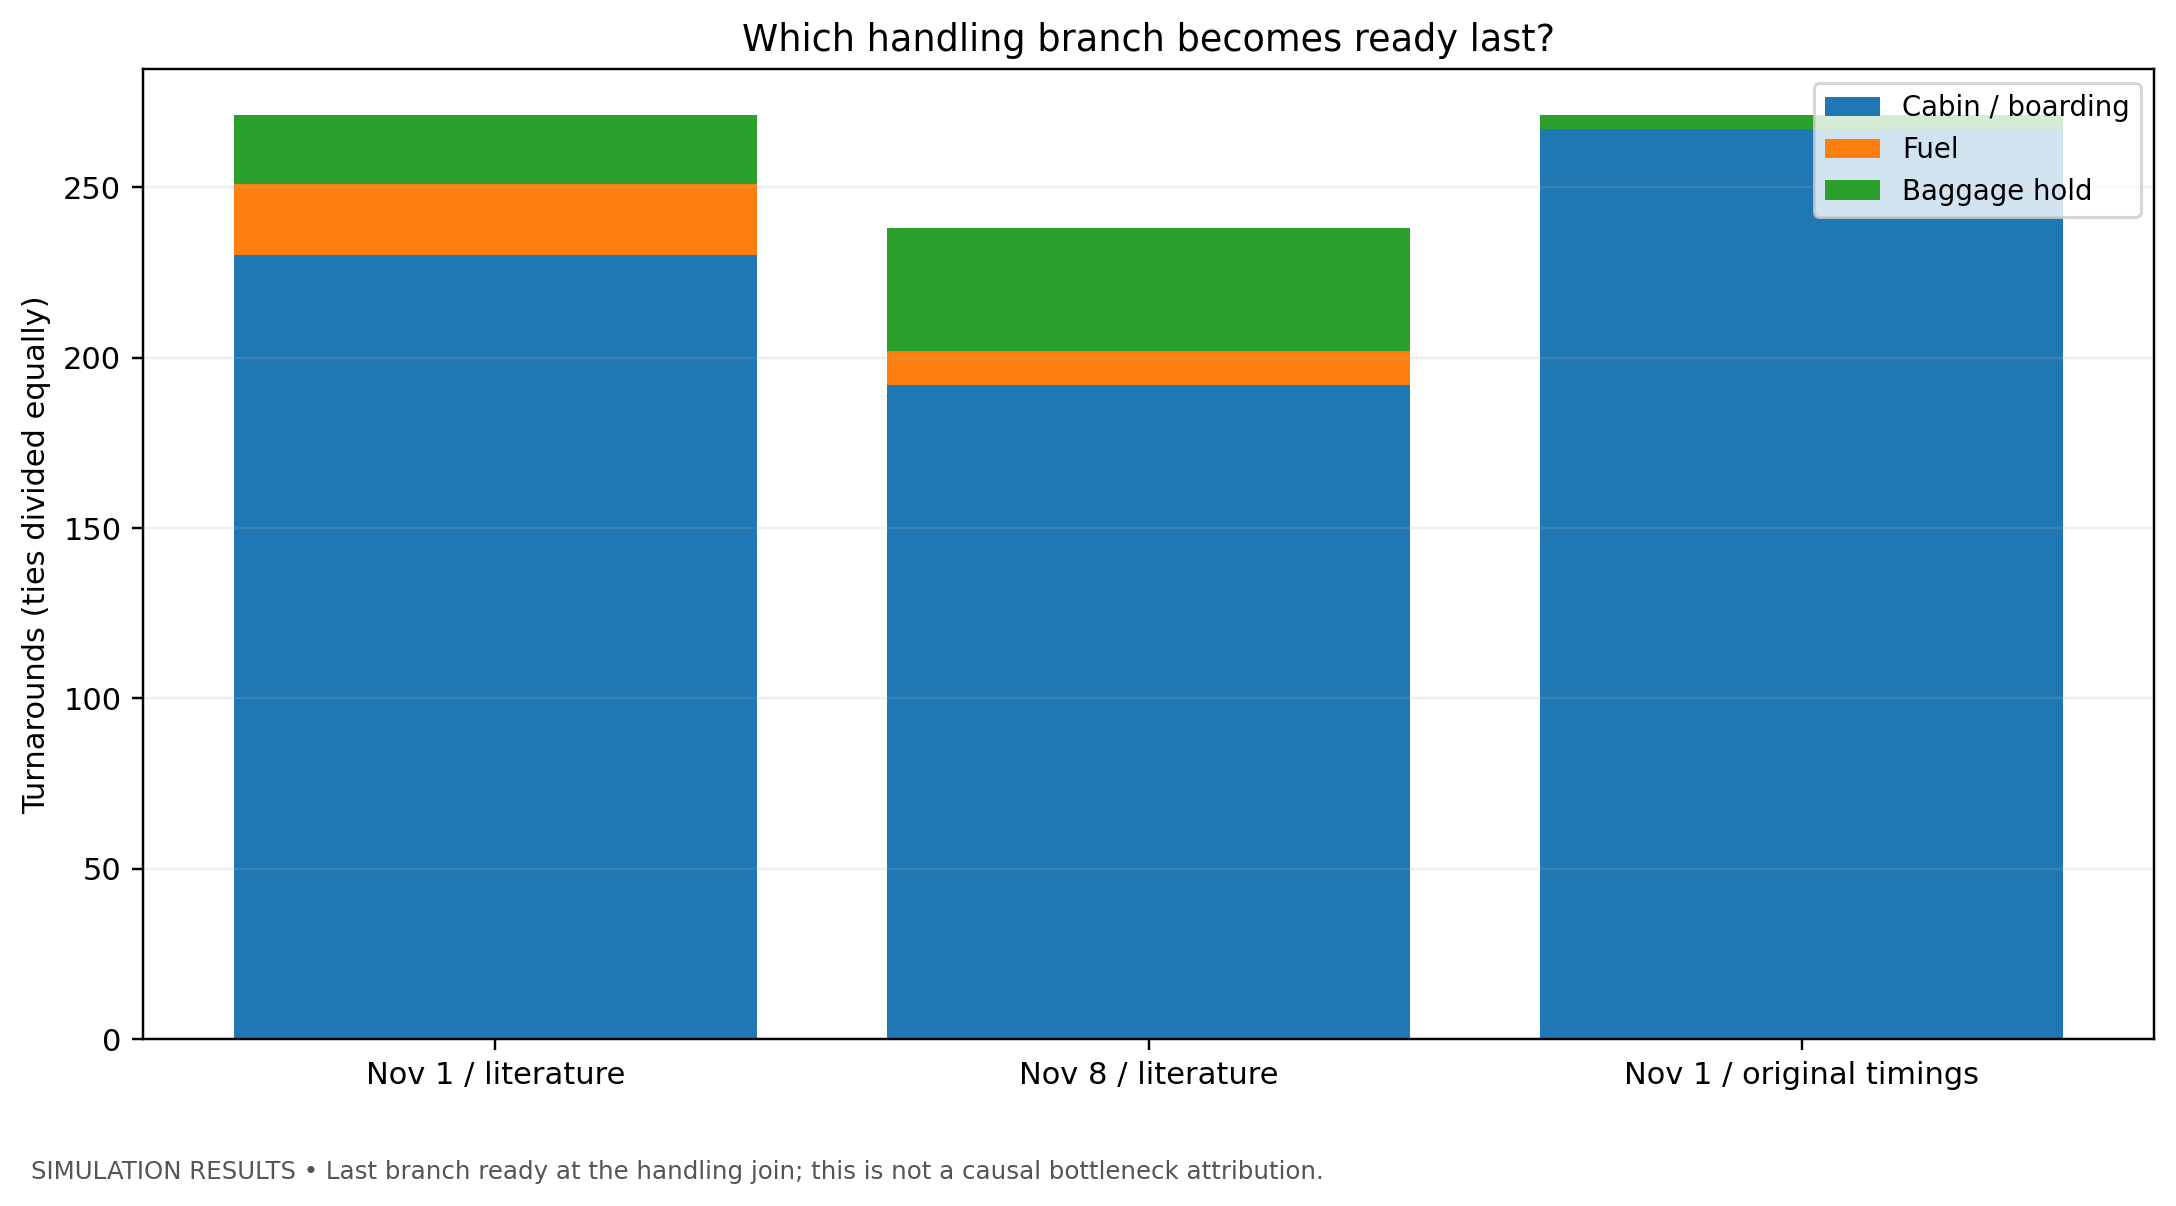
\includegraphics[width=\textwidth]{study_last_ready.png}
\caption{Last-ready handling branch in the original three simulation logs, calculated from output-token availability at the join. This supplementary Python figure uses exported events; it is not a Promenade-generated chart.}\label{fig:lastready}
\end{figure}

These observations partially address RQ2 by exposing parallel dependencies and resource contention within the simulation. They do not establish real terminal-versus-remote stand differences or quantify empirical inter-flight delay propagation. Workload counts per shared resource must also not be called time utilization without occupancy-duration calculations.

\section{Case-definition diagnostic}
The 1 November Promenade overview has two connected object components, with 94\% of objects in the largest. Reusable resources connect many rotations; a connected-component case definition would therefore merge most of the day. A leading Turnaround extraction returns 271 executions and 271 variants at the selected settings, but expanded executions can include shared-resource events. One expanded execution displays approximately 16.7 hours, which is not that turnaround's paired block duration. The analysis therefore uses direct paired milestones for duration statistics. A SQL-discovered object-centric directly-follows graph was produced; the separate metro-map layout was canceled after stalling and is not a completed result.

\section{Observed proxy discrepancies}
The first 1 November literature run has a simulated planned-arrival-to-takeoff proxy median of 79.63 minutes, close to the observed boundary-proxy median of 79.12. However, their means are 85.63 versus 156.17 minutes, with mean bias $-70.55$ minutes and mean absolute discrepancy 92.09 minutes. On 8 November, mean bias is $-101.60$ minutes and mean absolute discrepancy 116.00 minutes.
\begin{figure}[htbp]\centering
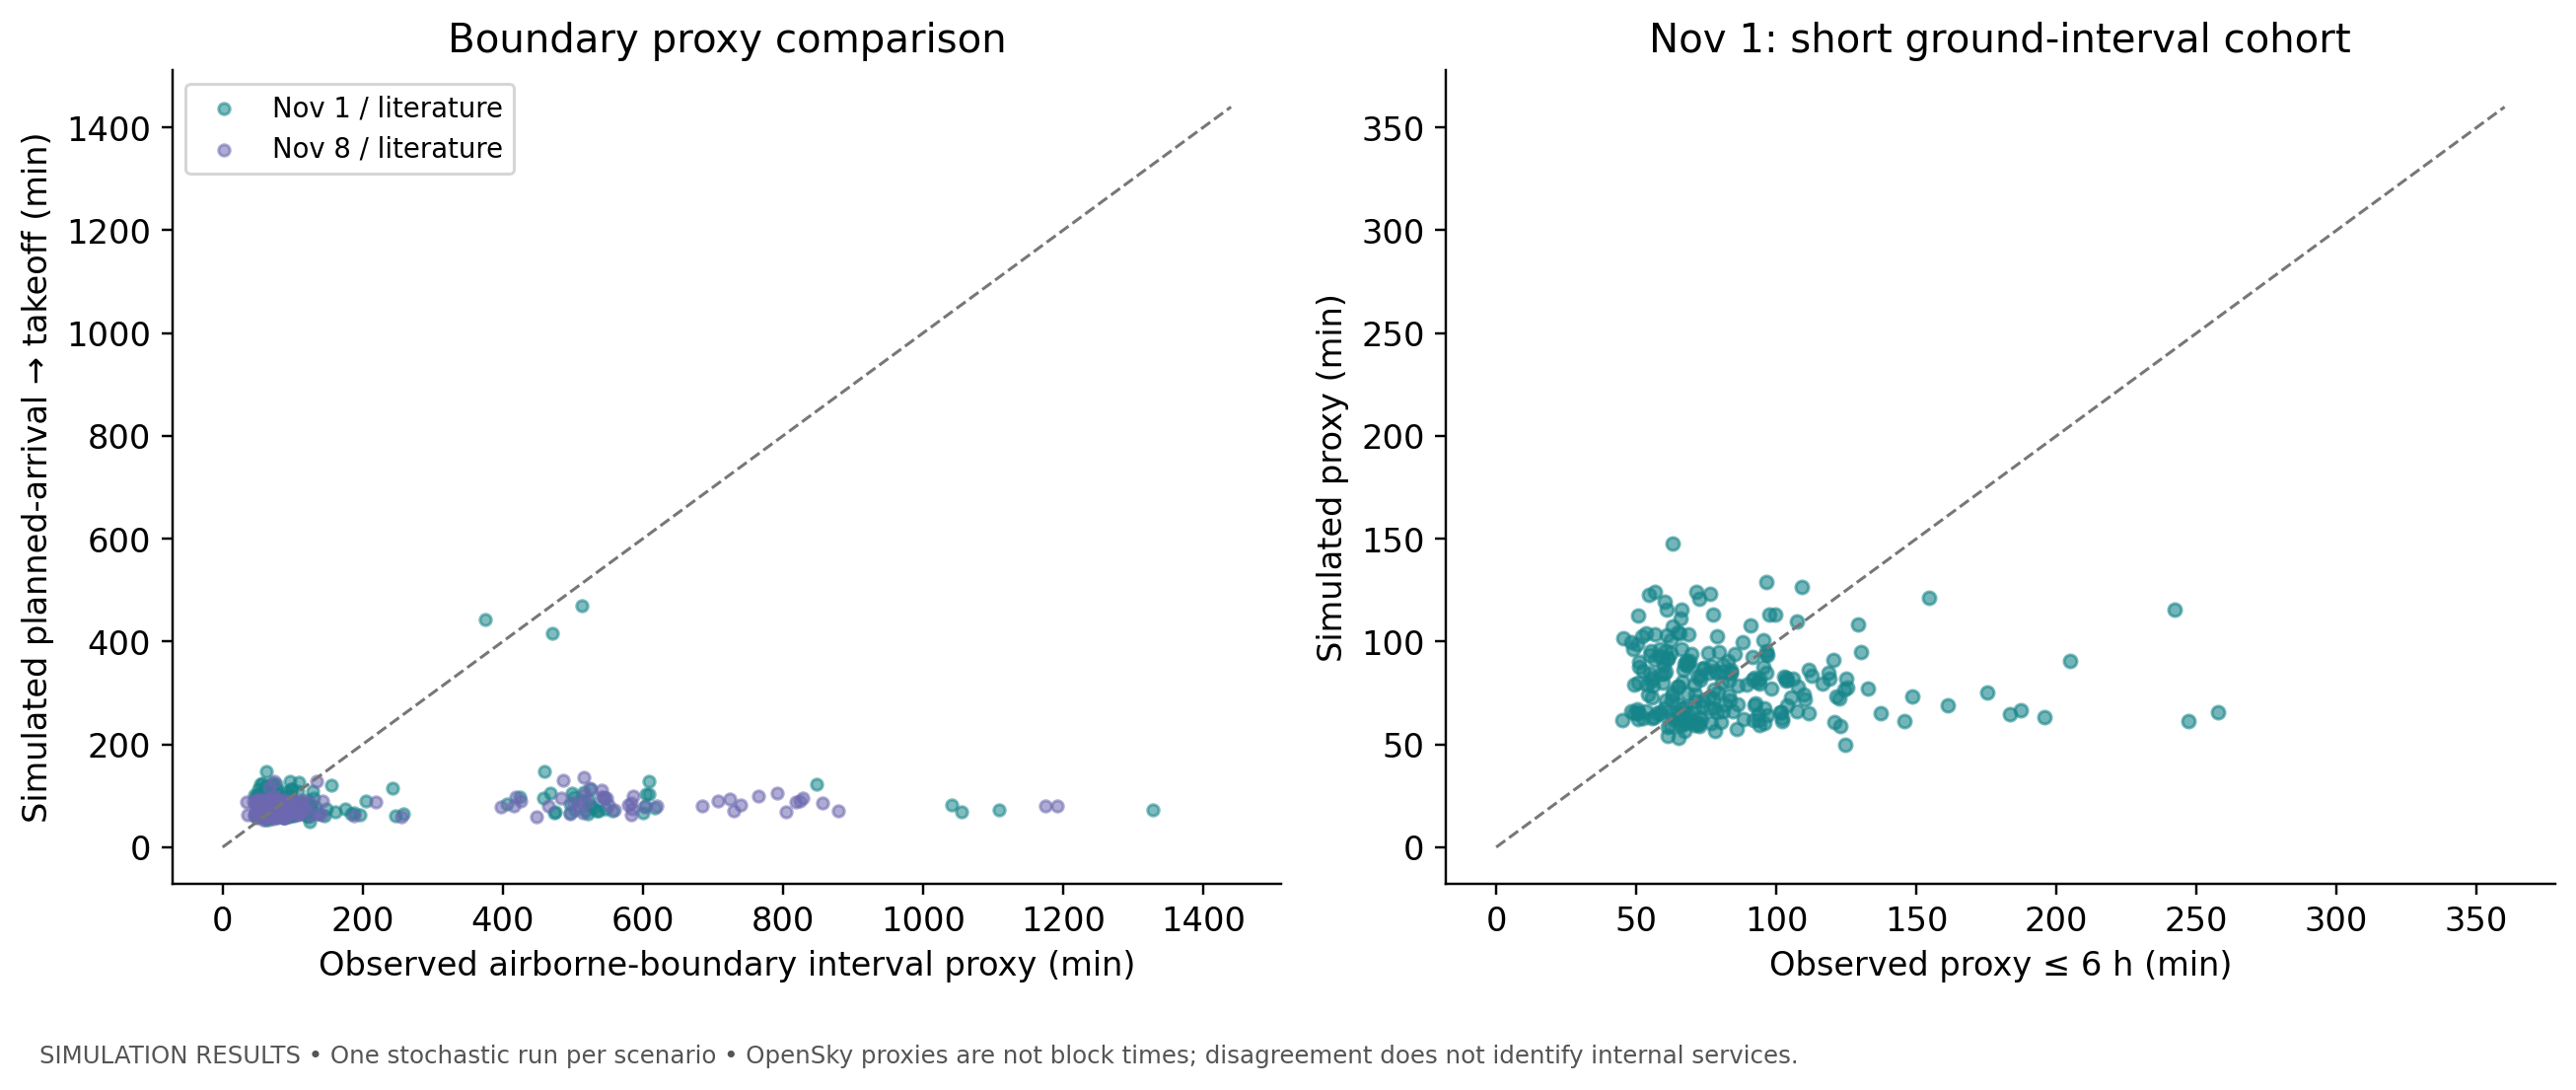
\includegraphics[width=\textwidth]{study_proxy_comparison.png}
\caption{Exploratory comparison with observed boundary proxies for the initial logs. These are not errors against measured AIBT--AOBT. Long stays and differing timestamp semantics limit interpretation.}\label{fig:proxy}
\end{figure}

A close median therefore conceals a poor distributional match. The current simulator starts handling after arrival and departs when ready, while observations can include parking and schedule buffers. Service durations should not be inflated merely to absorb that mismatch. Pairing review, stay stratification and independently justified departure scheduling are required before accuracy claims.

\section{Repeated timing and policy comparisons}
All 60 controlled runs complete and pass integrity checks. Table~\ref{tab:controlled} gives the mean of five replication means per date/scenario. Figure~\ref{fig:timing} shows the individual run means and intervals.
\begin{table}[htbp]\centering\small
\begin{tabular}{lrr}\hline
Scenario & Nov. 1 mean [95\% CI] & Nov. 8 mean [95\% CI]\\\hline
Original, inherited policy & 86.91 [84.83,89.00] & 72.73 [69.30,76.17]\\
Literature, inherited policy & 61.91 [59.82,64.01] & 59.22 [58.91,59.52]\\
Original, disabled curfew & 66.73 [66.14,67.32] & 66.07 [65.78,66.37]\\
Literature, disabled curfew & 59.20 [58.59,59.81] & 59.03 [58.45,59.61]\\
Six cleaning teams, disabled & 59.26 [58.39,60.13] & 59.20 [58.33,60.06]\\
Six+six fuel units, disabled & 58.58 [58.34,58.81] & 58.81 [58.56,59.06]\\\hline
\end{tabular}
\caption{Mean simulated block duration in minutes. Resource variants use literature timings; the reference has nine cleaning teams and four+four fuel units. Intervals quantify between-run simulation variability only.}\label{tab:controlled}
\end{table}
\begin{figure}[htbp]\centering
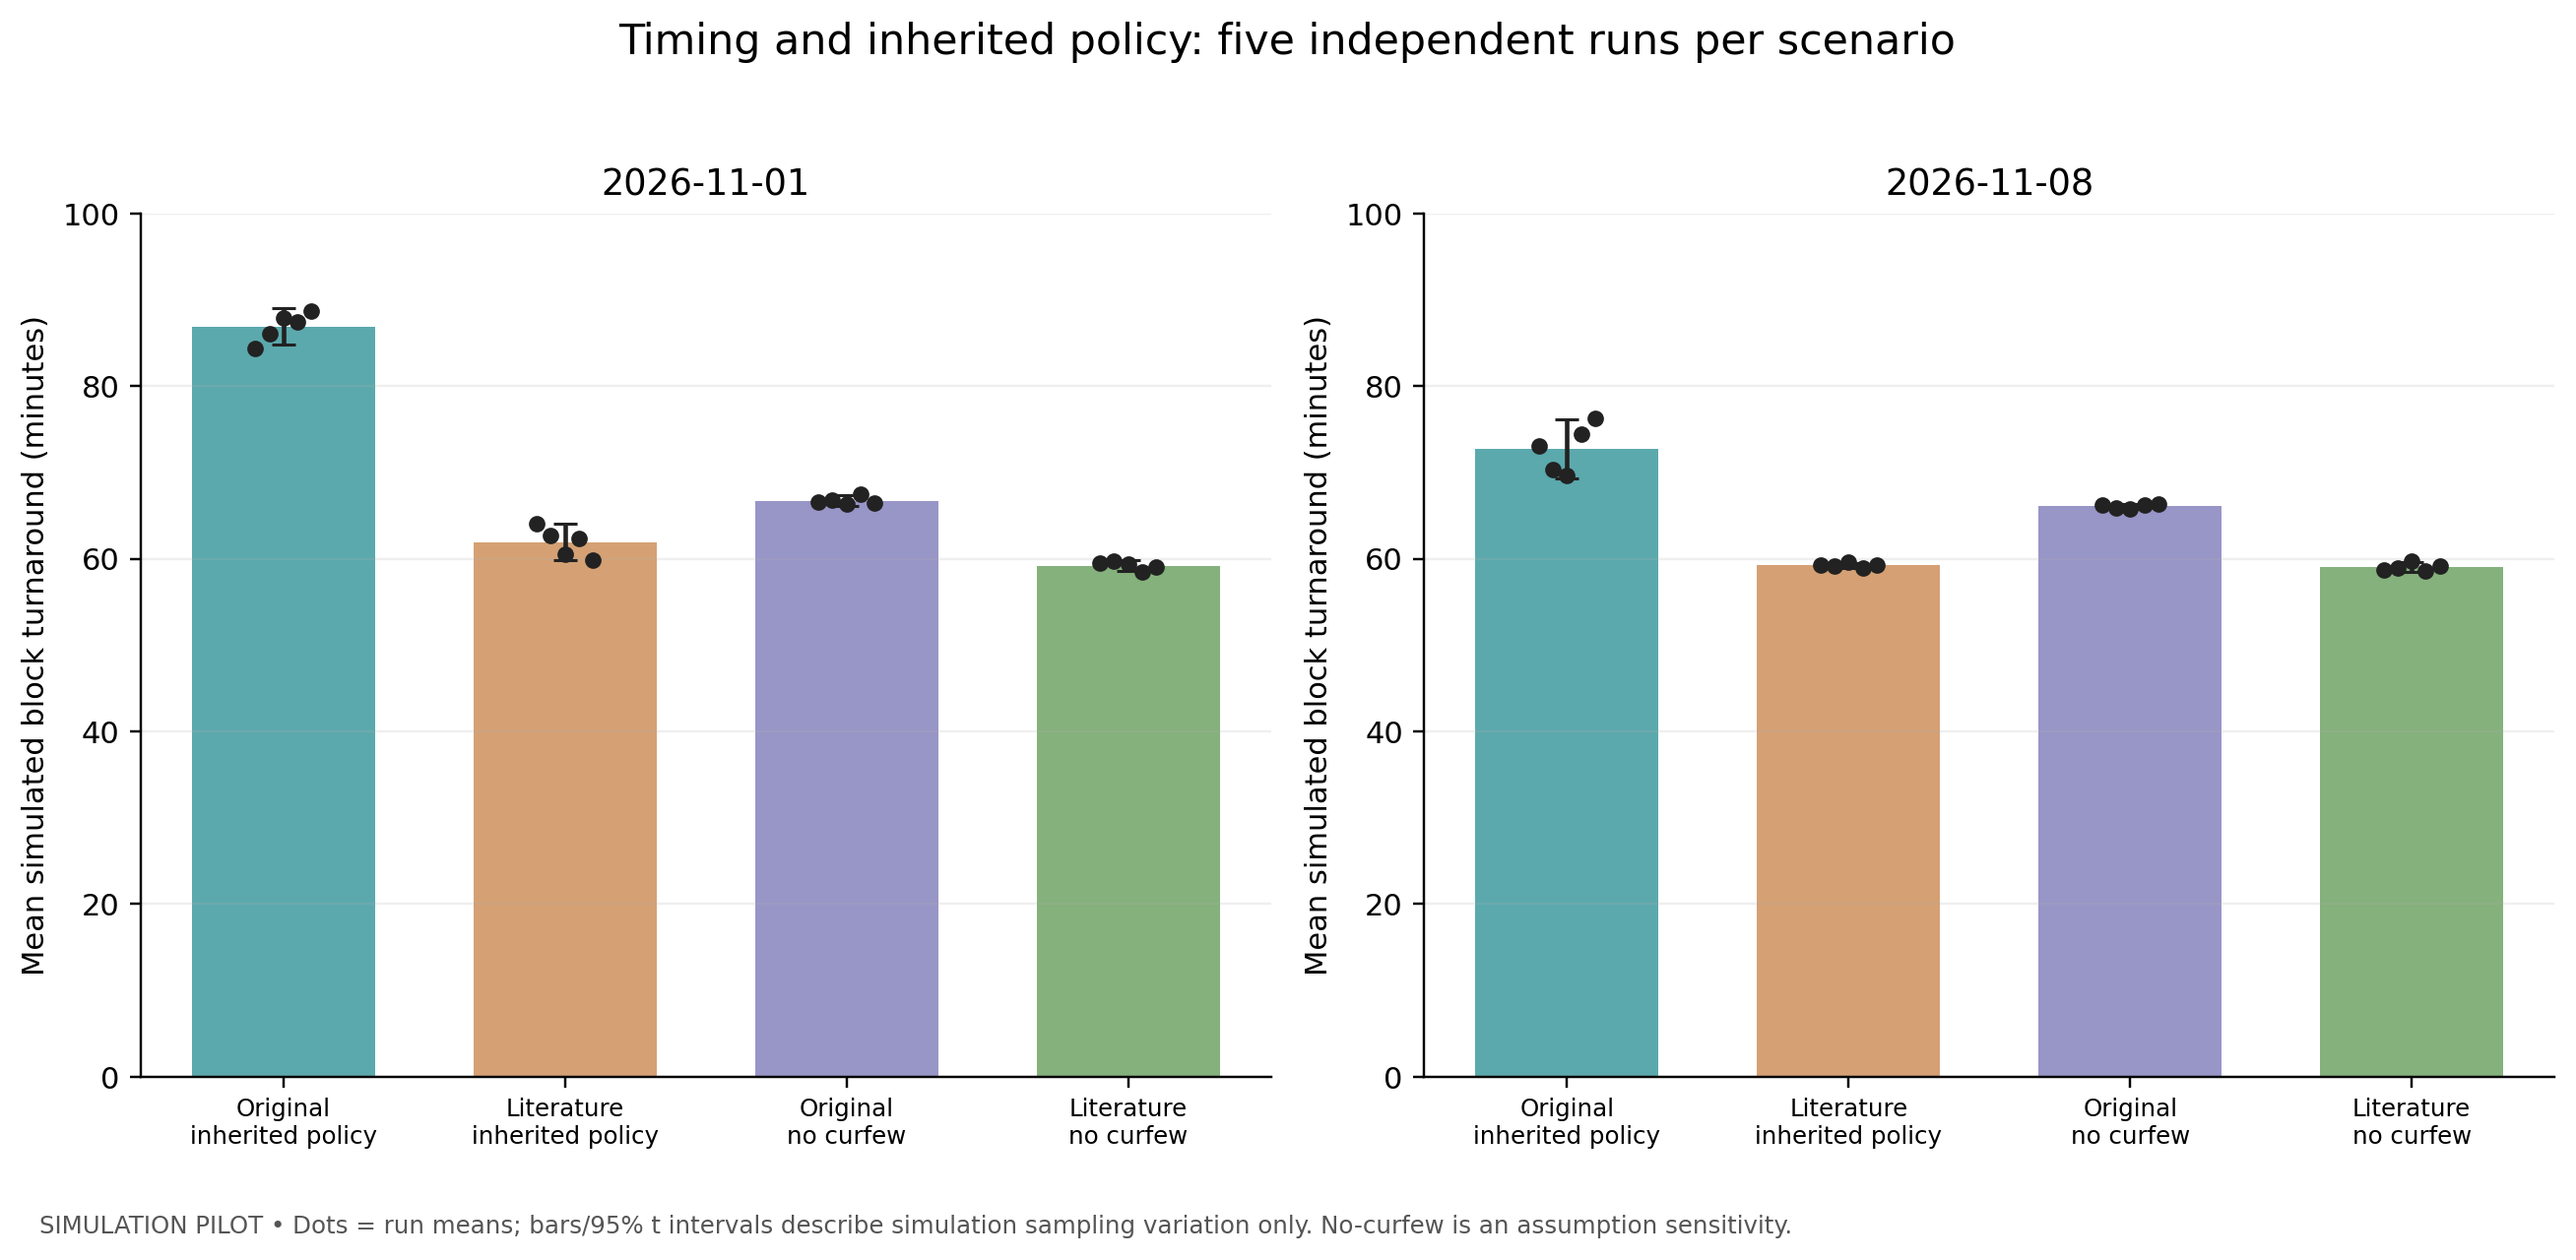
\includegraphics[width=\textwidth]{study_timing_policy.png}
\caption{Timing/policy comparisons: five independent run means per scenario, with Student-$t$ 95\% intervals. Disabled curfew is a diagnostic assumption sensitivity.}\label{fig:timing}
\end{figure}

With curfew disabled, literature-minus-original timing differences are $-7.53$ minutes on 1 November (Welch 95\% CI $[-8.24,-6.82]$) and $-7.04$ on 8 November ($[-7.62,-6.47]$). Under inherited policy the differences increase to $-25.00$ ($[-27.45,-22.54]$) and $-13.52$ ($[-16.94,-10.09]$). The apparent timing benefit therefore interacts strongly with policy logic; it is not evidence that transferred timings are more accurate.

An additional exploratory interaction contrast, added while inspecting the pilot, subtracts the disabled-curfew timing difference from the inherited-policy timing difference. Estimates are $-17.46$ minutes ($[-19.96,-14.97]$) and $-6.48$ ($[-9.88,-3.08]$). This is a conditional model finding, not a preregistered confirmatory result or a causal statement about airport regulations.

\section{Repeated resource sensitivity}
Under literature timings and disabled curfew, increasing fueling capacity from eight to twelve units reduces mean dispatch waiting from 3.042 to 0.168 minutes on 1 November and from 2.040 to 0.066 on 8 November. Final block-duration differences are much smaller: $-0.62$ minutes (95\% CI $[-1.23,-0.02]$) and $-0.22$ ($[-0.79,0.35]$). The latter interval crosses zero. A substantial queue reduction therefore does not establish a consistently substantial overall turnaround improvement.
\begin{figure}[htbp]\centering
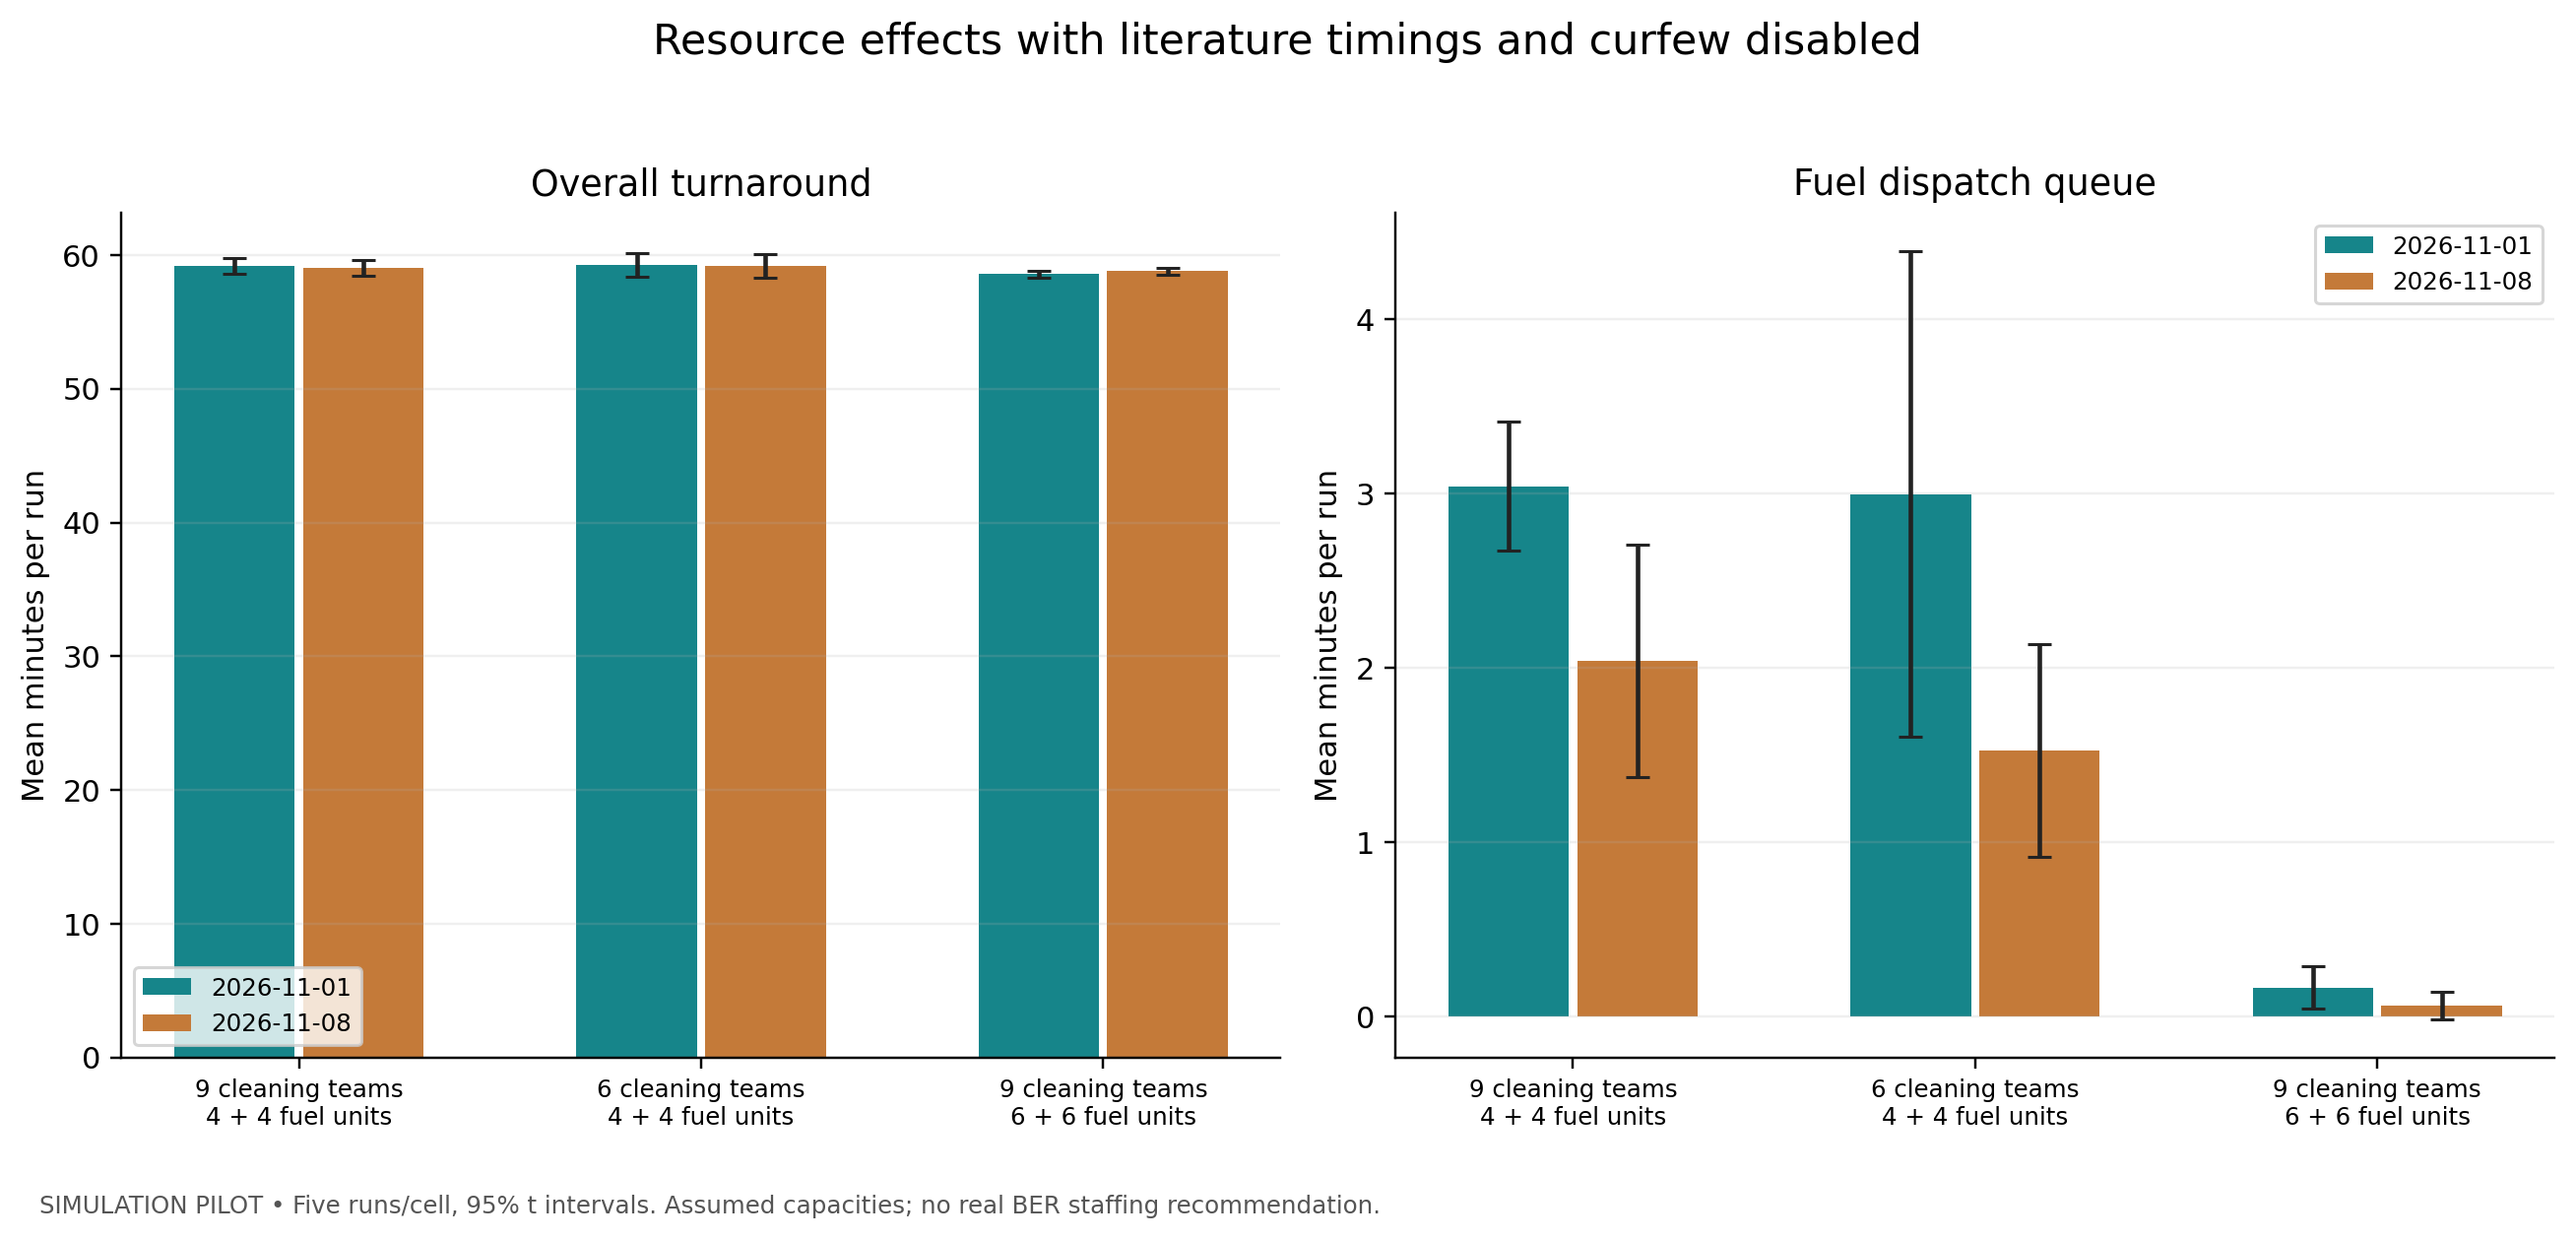
\includegraphics[width=\textwidth]{study_resource_sensitivity.png}
\caption{Resource sensitivity: overall turnaround and fuel-dispatch waiting respond differently. Counts are assumed model capacities, not verified BER staffing.}\label{fig:resource}
\end{figure}

Reducing cleaning teams from nine to six produces estimated block-duration increases of 0.07 minutes ($[-0.84,0.97]$) and 0.17 ($[-0.72,1.05]$). Neither comparison resolves a direction in this pilot. This is not a demonstration of equivalence or non-inferiority and does not justify a staffing reduction.
\begin{figure}[htbp]\centering
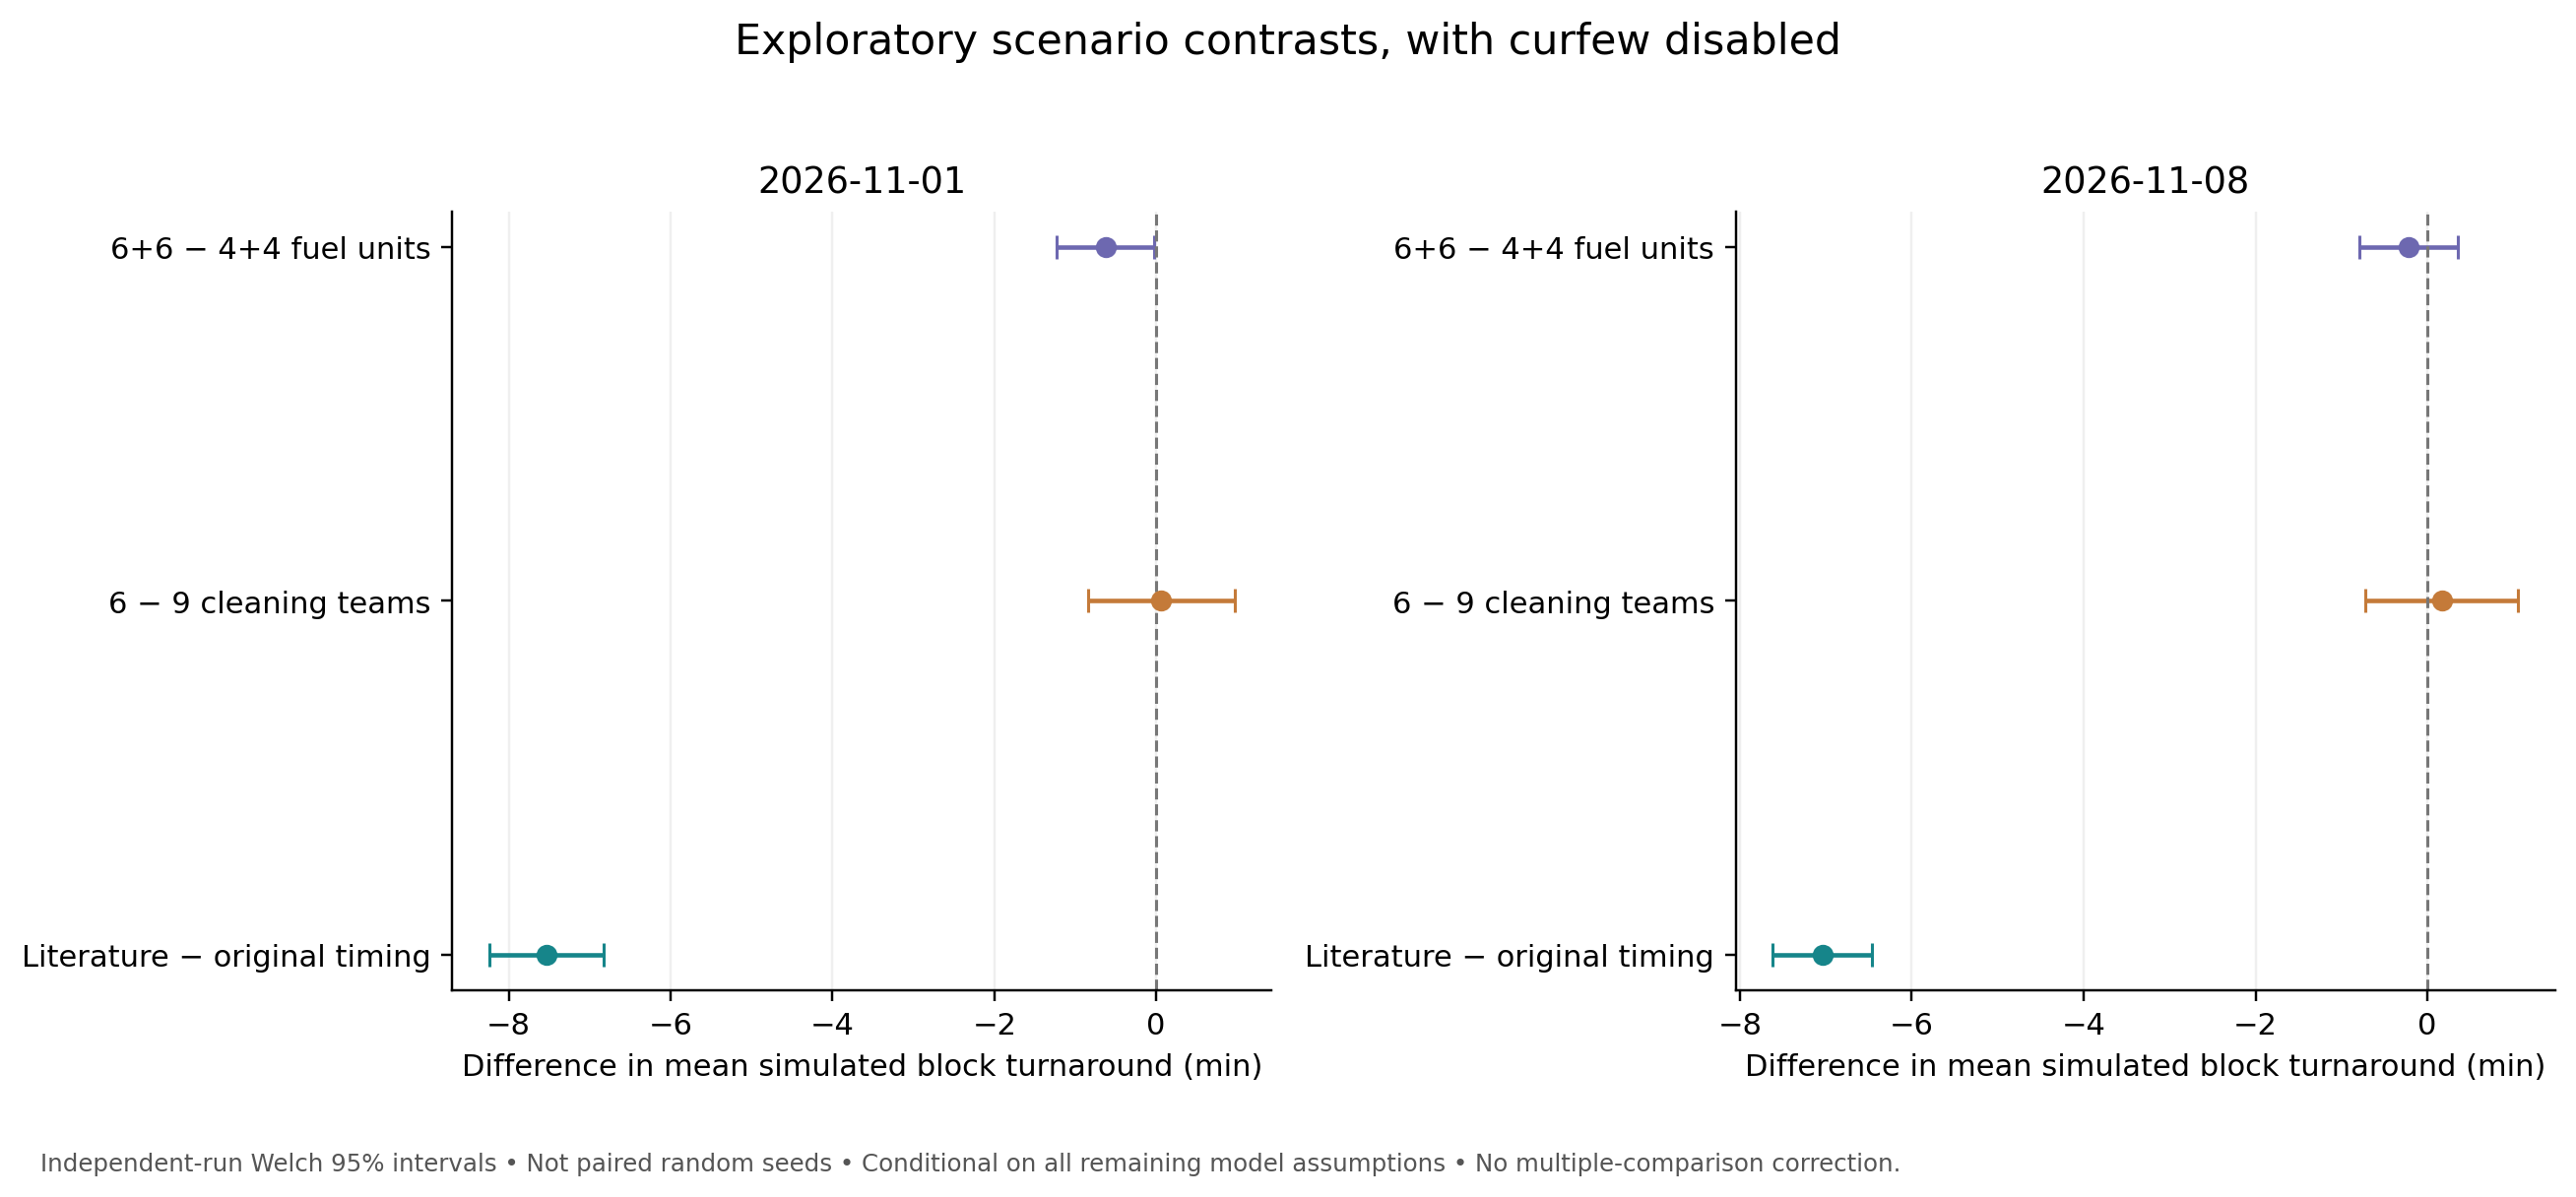
\includegraphics[width=\textwidth]{study_contrasts.png}
\caption{Exploratory independent-run Welch 95\% intervals for block-duration differences with curfew disabled. No multiplicity adjustment is applied.}\label{fig:contrasts}
\end{figure}

For RQ3, these scenarios demonstrate a functioning evaluation method and conditional trade-offs. They do not establish a cost-optimal configuration, compare alternative dispatch priorities, or optimize real BER resource allocation.
